\documentclass[a4paper]{article}

\usepackage[utf8]{inputenc}
\usepackage[T1]{fontenc}
\usepackage[spanish]{babel}
\usepackage[left=2cm, right=2cm, top=2cm, bottom=2cm]{geometry}
\usepackage{setspace}
\usepackage{graphicx}
\usepackage{xcolor}
\usepackage{geometry}
\usepackage{multirow}
\usepackage[hidelinks]{hyperref}
\usepackage{setspace} % Para el espaciado entre lineas
\setstretch{1.2} % Aquí definimos el espaciado en unidades
\usepackage{parskip} %  Para arreglar la forma en la que se manejan los parrafos
\usepackage{fancyhdr}
\usepackage{tikz,lipsum,lmodern}
\usepackage[most]{tcolorbox}
\usetikzlibrary{shapes.geometric, arrows}

% Sets de dimensiones
\setlength{\parindent}{0pt}
\setlength{\parskip}{0.8em plus 0.5em minus 0.2em}
\setlength{\parfillskip}{\parindent plus 1fill}

% Declaración de variables personalizadas
\newcommand{\logoPortada}{Images/PixelartPisa.png}
\newcommand{\cifplogo}{Images/cifplogo.png}

% Definición de colores
\definecolor{bluePortada}{HTML}{146c8a}

%Adicionales
\setlength{\headheight}{40.2pt}
\pagestyle{fancy}
\fancyhf{}
\lhead{\includegraphics[width=1cm]{\logoPortada}}\rhead{
\includegraphics[width=2cm]{Images/cifplogo.png}}
\renewcommand{\headrulewidth}{3pt}
\renewcommand{\headrule}{\hbox to\headwidth{\color{bluePortada}\leaders\hrule height \headrulewidth\hfill}}

\tikzstyle{startstop}=[rectangle,rounded corners, minimum width=3cm,minimum height= 1cm, text centered,draw=black, fill=red]
\tikzstyle{io}=[trapezium,trapezium left angle=70,trapezium right angle=110,minimum width=3cm,minimum height= 1cm, text centered,draw=black, fill=blue]
\tikzstyle{process}=[rectangle,minimum width=3cm,minimum height= 1cm, text centered,text width= 3cm,draw=black, fill=orange]
\tikzstyle{decision}=[diamond,minimum width=3cm,minimum height= 1cm, text centered,draw=black, fill=green]
\tikzstyle{arrow}=[thick]



\begin{document} % Inicio del documento
	\begin{titlepage}
		\centering % para centrar
		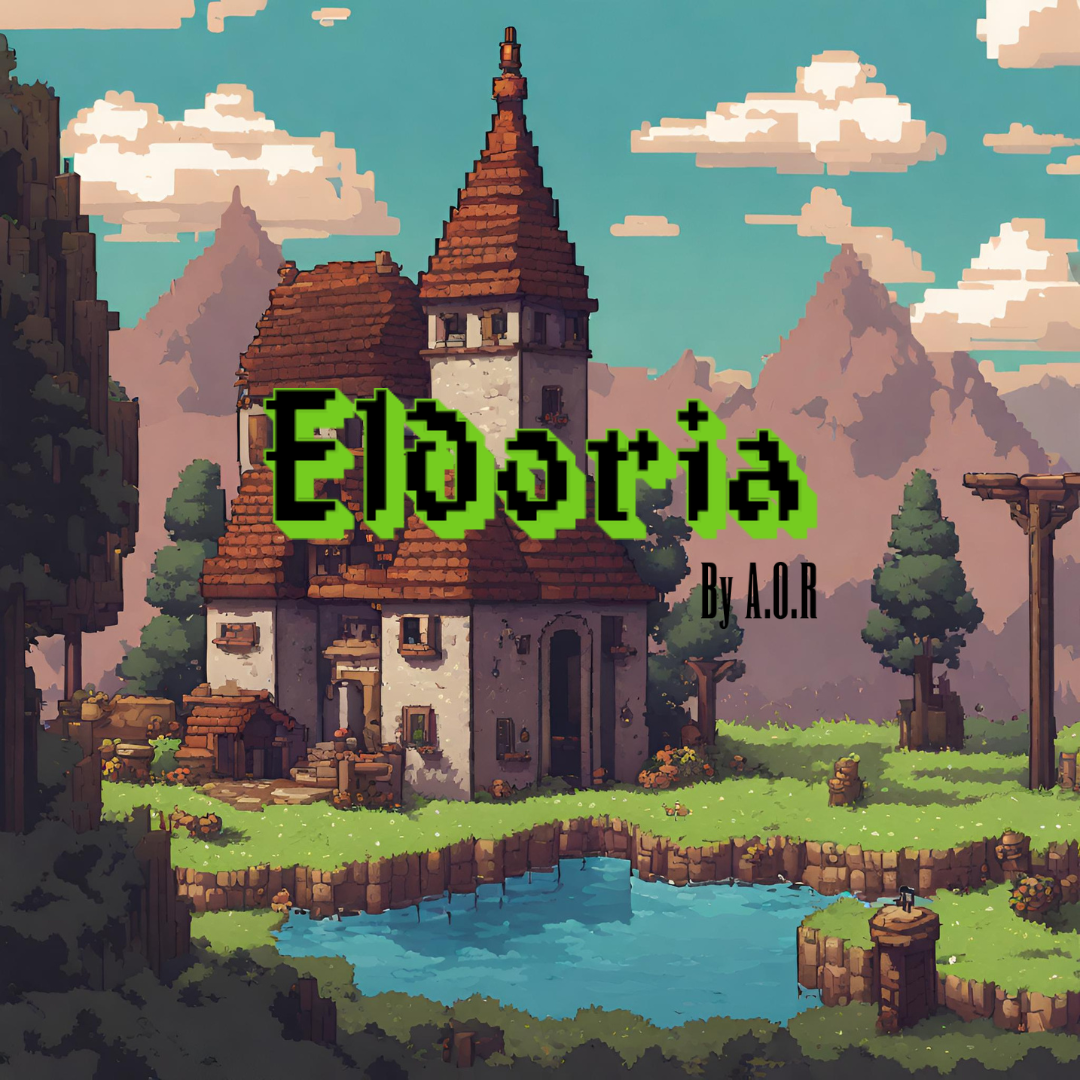
\includegraphics[width=0.5\textwidth]{Images/Eldoria.png}\par
		\vspace{0.4cm}
		{\scshape\LARGE\textbf{TFG DAM - CIFP LaLaboral}\par} % Contenido de la portada
		\vspace{0.4cm}
		{\LARGE\textcolor{bluePortada}{Eldoria - Alejandro Orviz Recalde}\par}
	\end{titlepage}
    % Comienzo del TOC
    \clearpage
    \tableofcontents
    \clearpage
    % ---------------------------------------------------------------------

    \section{Introducción}
    El presente proyecto trata sobre un Juego llamado \textbf{Eldoria}, se encuentra desarrollado en java y es una aventura en 2 dimensiones con graficos pixel art
    la cual tendra una forma de jugar similar a videojuegos antiguos tales como:
    \begin{itemize}
        \item The legend of Zelda
        \item The legend of Zelda Minish cap 
        \item Final Fantasy I, II, III
        \item Super Mario RPG
    \end{itemize}
    Algunos datos del proyecto adicionales son:

\begin{center}
    \begin{tabular}{| c | c |}
        \hline
        Titulo de la aplicacion & Eldoria \\ \hline
        Autor & Alejandro Orviz \\ \hline
        Profesor & Alberto \\ \hline
    \end{tabular}
\end{center}

    El videojuego se inspira fuertemente en los primeros juegos creados para la Super Nintendo, por lo que se veran bastantes similitudes tanto en estructura de niveles
    como en linealidad e historia del mismo. Ademas todas las images que se han usado son libres de derechos de autor.

    \clearpage
    % ----------------------------------------------------
    \section{Motivación}
    A dia de hoy son muchas las personas que juegan a videojuegos, pero no mucho recuerdan las bases u origenes de los mismos, en este caso, en mi juego llamado
    \textbf{Eldoria} tenemos un juego en 2 dimensiones en estetica pixel que nos lleva a un mundo de fantasia el cual nos puede provocar la nostalgia de revivir
    videojuegos como The legend of Zelda 1. Ademas este videojuego aprovecha conceptos de programacion sobre lectura, apertura y creacion de archivos asi como 
    conexiones con bases de datos. La duracion del mismo aun esta por determinar y depende mas bien de la persona y del tipo de jugador. Con este proyecto se busca
    es proveer al usuario de un tiempo de ocio en el que pueda disfrutar pasando el tiempo frente a retos y acertijos propuestos por el videojuego.
    \clearpage
    %-----------------------------------------------------
    \section{Objetivos del videojuego}
    \begin{enumerate}
        \item \textbf{Recuperar la Llave del Destino:}
            \begin{itemize}
                \item Explora los diversos templos y mazmorras dispersos por Eldoria para localizar los tres fragmentos de la Llave del Destino.
                \item Supera desafiantes enemigos y resuelve intrincados rompecabezas para acceder a cada fragmento.
            \end{itemize}
    
        \item \textbf{Desafiar a las Fuerzas Oscuras:}
            \begin{itemize}
                \item Enfrenta hordas de criaturas místicas y jefes desafiantes que han sido corrompidos por la oscuridad.
                \item Utiliza tu habilidad con la espada y descubre nuevas armas mágicas para derrotar a Morvath y sus secuaces.
            \end{itemize}
    
        \item \textbf{Explorar Eldoria:}
            \begin{itemize}
                \item Viaja a través de vastos paisajes, desde bosques encantados hasta desiertos desolados, en tu búsqueda por la Llave del Destino.
                \item Interactúa con aldeanos y personajes intrigantes para obtener pistas y misiones secundarias.
            \end{itemize}
    
        \item \textbf{Potenciar al Héroe:}
            \begin{itemize}
                \item Encuentra mejoras para tu personaje, como corazones adicionales y artefactos mágicos, que te otorgarán nuevas habilidades y resistencia en la batalla.
                \item Desbloquea áreas previamente inaccesibles a medida que fortaleces a tu héroe.
            \end{itemize}
    
        \item \textbf{Restaurar la Paz en Eldoria:}
            \begin{itemize}
                \item Une los fragmentos de la Llave del Destino y enfrenta a Morvath en un enfrentamiento épico.
                \item Libera a Eldoria de la oscuridad y restaura el equilibrio en el reino.
            \end{itemize}
    
        \item \textbf{Completa Misiones Secundarias:}
            \begin{itemize}
                \item Ayuda a los aldeanos con sus problemas y busca tesoros ocultos para obtener recompensas adicionales.
                \item Descubre secretos y leyendas mientras exploras cada rincón de Eldoria.
            \end{itemize}
    
        \item \textbf{Construir un Legado:}
            \begin{itemize}
                \item Deja tu marca en Eldoria al completar desafíos opcionales y objetivos extra.
                \item Desbloquea escenas finales y descubre el impacto de tus acciones en el destino del reino.
            \end{itemize}
    \end{enumerate}

    \clearpage
    % --------------------------------------------
    \section{Objetivos planteados}
    \begin{enumerate}
        \item \textbf{Manejo de estructuras logicas}
        \item \textbf{Manejo de datos en una bdd a traves de un programa Java}
        \item \textbf{Mejora de las habilidades como programador}
    \end{enumerate}
    \clearpage
    % --------------------------------------------
    \section{Estudio de mercado y viabilidad de la propuesta}
    \subsection{Aplicaciones ya existentes}
    Este tipo de videojuego ya existe, siendo claros ejemplos, \textbf{Final Fantasy 1}, \textbf{The legend of Zelda} o incluso \textbf{Pokemon rojo}, este tipo de
    programas que han sido desarrollados hace años tienen en común que siguen la estética \textit{pixel art} y en ellos se entiende ya que por circunstancias temporales,
    no existía nada mejor. En este caso son ejemplos válidos \textit{Sea of stars} el cual fue lanzado en el año 2023, siguiendo tambien una estetica \textit{retro}, y tambien siguiendo
    un genero parecido a los juegos ya mencionados.
    \subsection{Viabilidad}
    Dentro de este proyecto nos enfrentamos a varios obstaculos y decisiones que nos van a hacer tardar mas o tardar menos en desarrollar el proyecto.
    Los principales obstaculos que nos hemos encontrado han sido:
    \begin{itemize}
        \item \textbf{Desconocimiento de la lógica de un videojuego:} \\
        La principal dificultad de este punto ha sido la poca familiaridad de la creacion de un programa que funcione como un videojuego, ya que se requiere una logica distinta a la que estoy familiarizado.
    
        \item \textbf{Desconocimiento en LaTeX:} \\
        A pesar de haber escogido LaTex para realizar el documento, el principal obstaculo ha sido tener en cuenta casi todos los aspectos de formato bonito para el documento, ya que la falta de experiencia
        documentando en LaTeX ha hecho complicado poder seguir de forma fluida el proyecto

        \item \textbf{Desconocimiento en la gestión de memoria:} \\
        La gestión de memoria es crucial en el desarrollo de software. La falta de entendimiento de este aspecto nos ha provocado un problema de rendimiento en las etapas tempranas del desarrollo.
    
        \item \textbf{Diseño de niveles:} \\
        En el caso de este punto ya que carecemos de teoria acerca de niveles se ha hecho complicado poder realizar un mapa competente ya que carece de una tecnicidad o complejidad excesiva.
       
        \item \textbf{Diseño de personajes:} \\
        En cuanto a los personajes se ha optado por usar galerias gratuitas, el principal obstaculo ha sido cuadrar los sprites ya que cada uno viene de autores diferentes y no puede quedar todo diferente.
        
        \item \textbf{Implementación de base de datos:} \\
        El principal problema de la Implementación de la base de datos, ha sido el que guardamos en la base de datos, ya que no podemos guardar algo que se tenga que consultar cada poco, por que provocaria
        en este caso problemas de rendimiento.

        \item \textbf{Desconocimiento de herramientas:} \\
        Uno de los principales problemas y lastres a la hora del desarrollo es el hecho de no contar con las suficientes herramientas, ya sea para diseñar niveles, personajes, o automatizar procesos

    \end{itemize}

    \subsection{Calendario del proyecto}
    \begin{table}[ht]
        \centering
        \begin{tabular}{|c|c|c|c|}
        \hline
        \textbf{Tarea} & \textbf{Fecha de Inicio} & \textbf{Fecha de Fin} & \textbf{Horas Planificadas} \\
        \hline
        Diseño de Juego & 20/08/2023 & 07/02/2024 & 20 \\
        \hline
        Desarrollo de Funcionalidades & 08/02/2024 & 28/02/2024 & 40 \\
        \hline
        Pruebas y Depuración & 01/03/2024 & 15/03/2024 & 30 \\
        \hline
        Diseño de Niveles & 10/01/2024 & 10/01/2024 & 15 \\
        \hline
        Apartado artistico de personajes & 04/10/2024 & 10/04/2024 & 25 \\
        \hline
        Documentación & 10/09/2023 & 30/04/2024 & 20 \\
        \hline
        \multicolumn{3}{|r|}{\textbf{Total de Horas Planificadas}} & \textbf{150} \\
        \hline
        \end{tabular}
        \label{tab:planificacion-horas}
    \end{table}

    
    \clearpage
    % -------------------------------------------
    \section{Requisitos de la aplicacion}
    Dentro de esta aplicacion no necesitamos tampoco unos requisitos muy avanzados, pero aun asi dejaremos anotados ciertos requisitos minimos y recomendados
    \subsection{Requisitos Mínimos}

\begin{itemize}
    \item \textbf{Procesador (CPU)}: Procesador de al menos 1.0 GHz.
    \item \textbf{Memoria RAM}: 1 GB de RAM.
    \item \textbf{Tarjeta Gráfica (GPU)}: Tarjeta gráfica integrada o dedicada capaz de manejar gráficos 2D simples.
    \item \textbf{Almacenamiento}: 100 MB de espacio libre en disco.
    \item \textbf{Sistema Operativo}: Windows 7/8/10, macOS 10.10 o superior, Linux con kernel 2.6 o superior.
\end{itemize}

\subsection{Requisitos Recomendados}

\begin{itemize}
    \item \textbf{Procesador (CPU)}: Procesador de doble núcleo de al menos 2.0 GHz.
    \item \textbf{Memoria RAM}: 2 GB de RAM.
    \item \textbf{Tarjeta Gráfica (GPU)}: Tarjeta gráfica integrada o dedicada para gráficos 2D mejorados.
    \item \textbf{Almacenamiento}: 500 MB de espacio libre en disco.
    \item \textbf{Sistema Operativo}: Windows 10, macOS 10.14 o superior, Linux con kernel 4.0 o superior.
\end{itemize}



    \clearpage
    % -------------------------------------------



    \section{Alcance}
    El videojuego final tratara de ser una aventura corta en la cual en una hora o dos de juego se llegue a completar, tambien se pondran \textit{easter eggs} para los jugadores mas curiosos, tambien el juego contara en principio
    con 3 niveles, uno introductorio, un segundo de una dificultad intermedia, y el ultimo sera mas complicado, es decir, habra 3 mapas jugables, tambien habra objetos y una tienda en la que el jugador podra comprar por ejemplo pociones.
    \subsection{Modos de juego}
    Solo existira un modo de juego el cual sera el de un solo jugador, no hay planes futuros de una posible actualizacion acerca de multijugador. 
    \subsection{Situacion actual}
    Actualmente disponemos de una version de un videojuego hecho en consola que funciona sin interfaz, es decir por consola a traves de texto,
    contamos con este videojuego el cual posee cierta logica de juego que nos puede servir de utilidad para el proyecto descrito.
    
    \clearpage
    % ------------------------------------------------
\section{Fases de desarrollo}

\subsection{Idea y concepto}
Esta fase es la conocida lluvia de ideas en la cual ponemos sobre la mesa todo lo que hemos pensado referente a un proyecto
\subsection{Diseño}
Aqui nos ponemos a pensar acerca de como seran los niveles, que niveles pensamos hacer, como sera el personaje, cosas mas bien esteticas
\subsection{Implementacion}
Dentro de esta fase ya empieza el desarrollo de codigo sobre el juego con la idea clara
\subsection{Testing}
Dentro de esta fase nos pondremos a intentar romper el juego provocar excepciones y ver que cosas fallan
\subsection{Refinamiento}
Esta fase tambien se puede llamar fase de optimizacion, en ella tomamos en cuenta lo visto en la fase de testeo y tratamos de hacer un codigo mas optimizado
\subsection{Salida del juego}
Fase final en la que ya lanzamos el juego completo

Aunque las fases son realmente consecutivas, quitando la ultima fase, lo que haremos es repetir en ciclo las demas fases.    

\clearpage
% -----------------------------------
\section{Arquitectura fisica}
\subsection{Plataforma de desarrollo}
En mi caso usare IntelliJ IDEA, debido a la rica cantidad de plugins que tiene y la facilidad de uso, ademas de que es un IDE muy completo en terminos de herramientas y ayuda mucho al programador a la hora de refactorizar.
\clearpage
% -----------------------------------
\section{Arquitectura logica}
\subsection{Diagrama de clases}
% metemos la imagen de la carpeta images que se llama diagrama.png
\begin{figure}[ht]
    \centering
    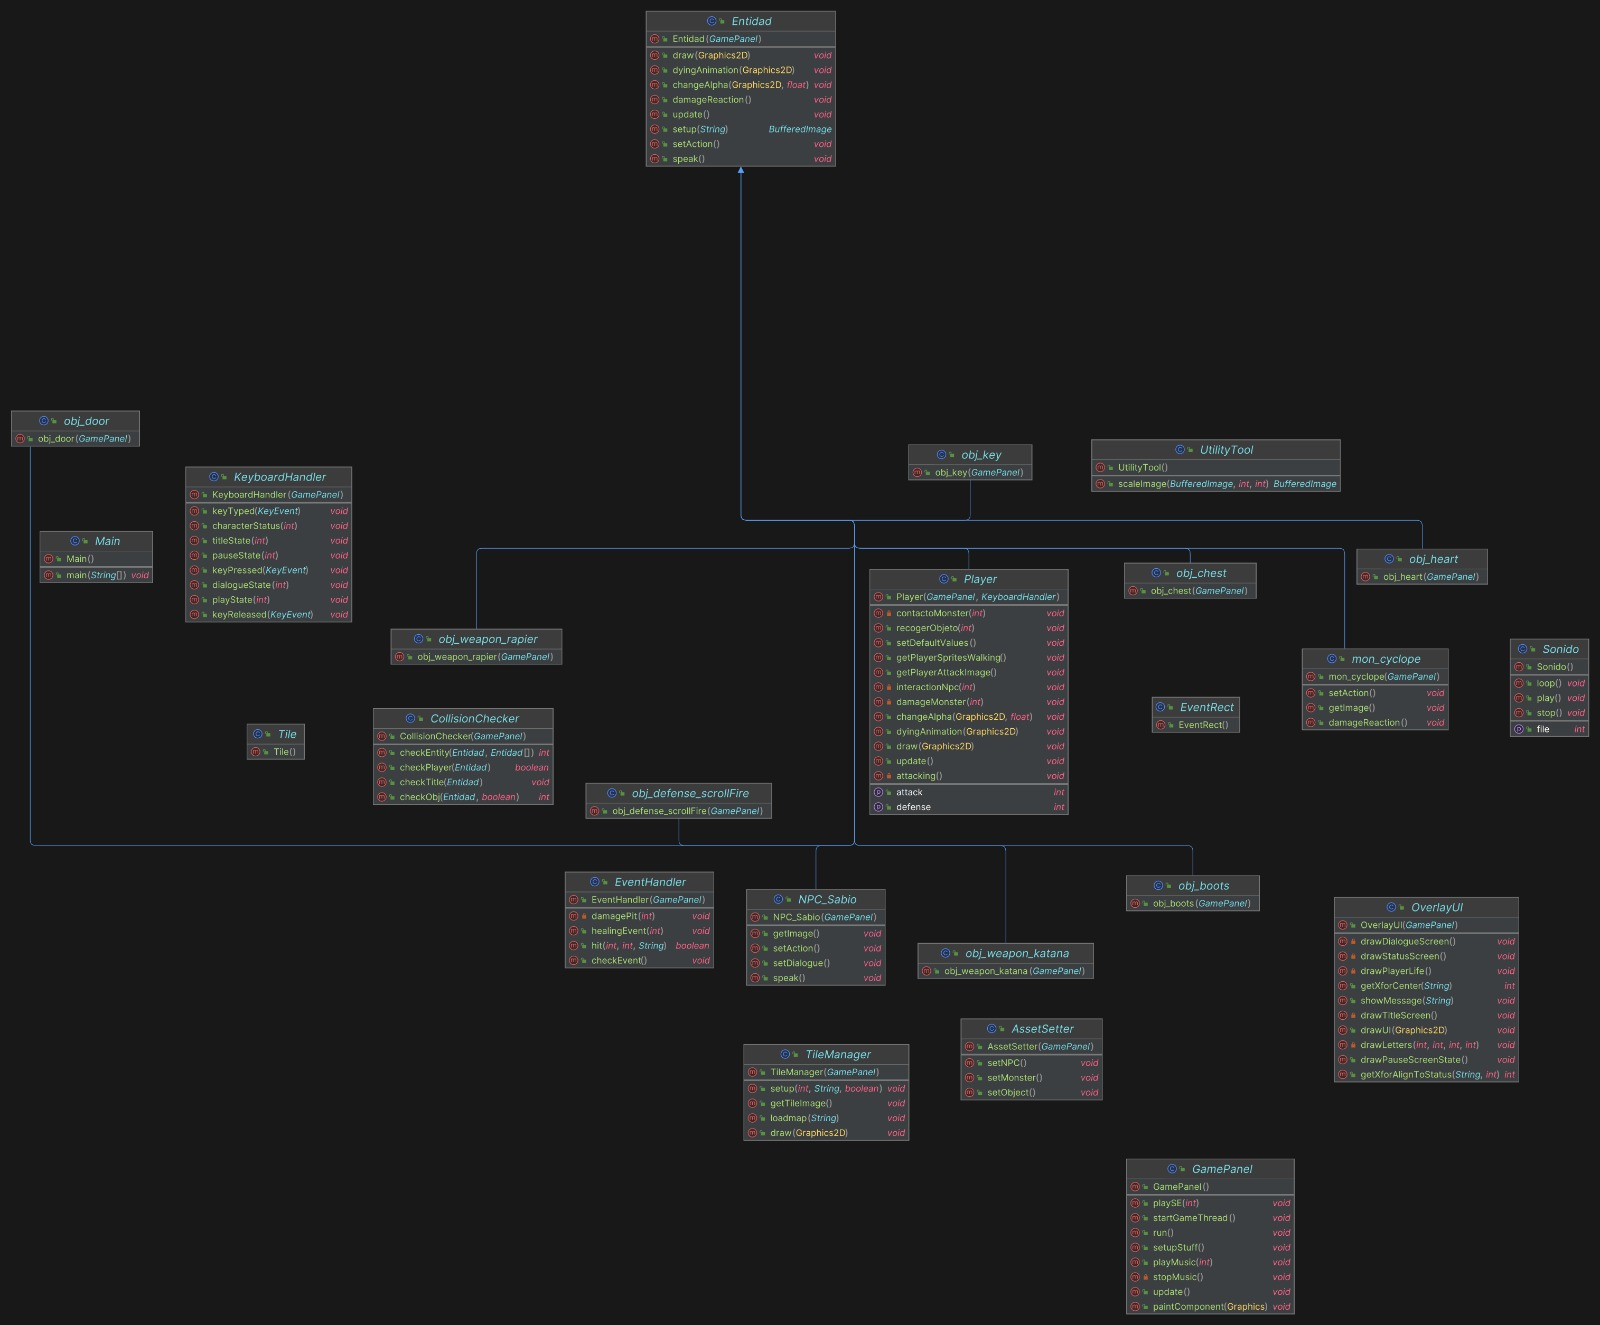
\includegraphics[width=0.8\textwidth]{Images/diagrama.png}
    \caption{Diagrama de clases}
    \label{fig:diagrama-clases}
\end{figure}
Una nota importante sobre este diagrama es que se trata de una version prematura del mismo, ya que se pondran nuevas clases y metodos que nos serviran de utilidad para el mismo.
\clearpage
% -----------------------------------
\section{Bibliografia}
% Haz un listado de las fuentes que has usado para realizar el proyecto
\begin{itemize}
    \item \textbf{Excalidraw} - \url{https://excalidraw.com/}
    \item \textbf{Manual LaTeX} - \url{https://manualdelatex.com/}
    \item \textbf{Mermaid} - \url{https://mermaid.js.org/intro/getting-started.html}
    \item \textbf{IntelliJ} - \url{https://www.jetbrains.com/es-es/idea/}
    \item \textbf{Pixelart} - \url{https://www.piskelapp.com/}
    \item \textbf{Como hacer Assets} - \url{https://tips.clip-studio.com/es-es/articles/2484}
    
\end{itemize}
\end{document}